% Created by tikzDevice version 0.6.2-92-0ad2792 on 2013-03-23 22:55:53
% !TEX encoding = UTF-8 Unicode
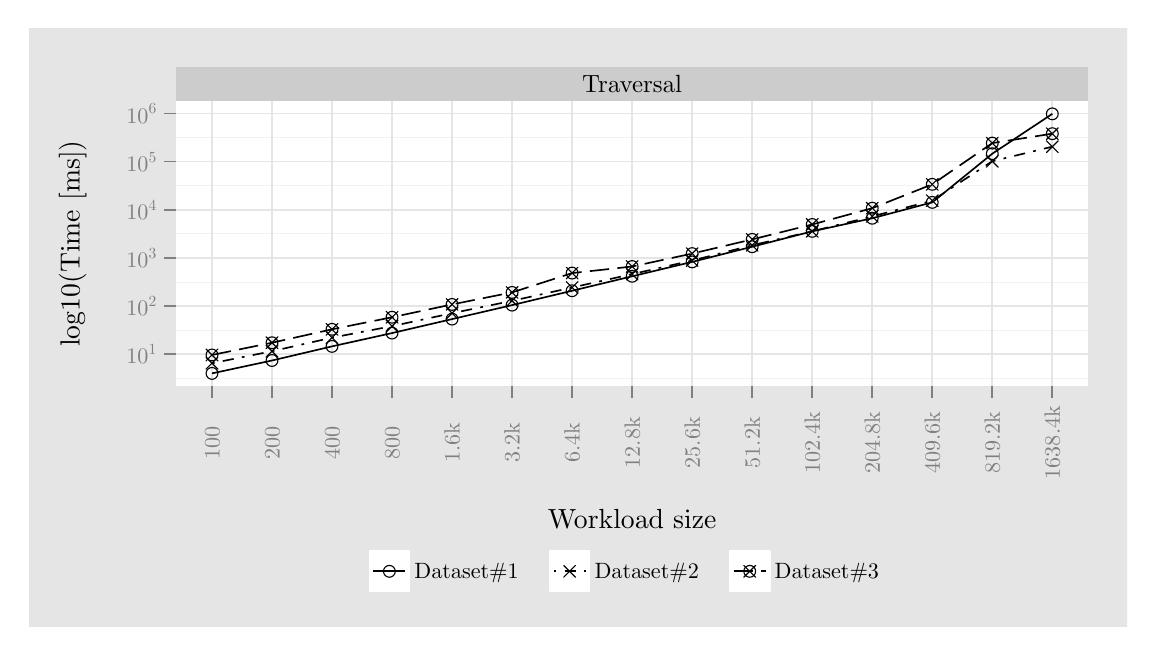
\begin{tikzpicture}[x=1pt,y=1pt]
\definecolor[named]{fillColor}{rgb}{1.00,1.00,1.00}
\path[use as bounding box,fill=fillColor,fill opacity=0.00] (0,0) rectangle (397.48,216.81);
\begin{scope}
\path[clip] (  0.00,  0.00) rectangle (397.48,216.81);
\definecolor[named]{drawColor}{rgb}{1.00,1.00,1.00}
\definecolor[named]{fillColor}{rgb}{0.90,0.90,0.90}

\path[draw=drawColor,line width= 0.6pt,line join=round,line cap=round,fill=fillColor] (  0.00,  0.00) rectangle (397.48,216.81);
\end{scope}
\begin{scope}
\path[clip] ( 53.58, 87.19) rectangle (383.26,190.36);
\definecolor[named]{fillColor}{rgb}{1.00,1.00,1.00}

\path[fill=fillColor] ( 53.58, 87.19) rectangle (383.26,190.36);
\definecolor[named]{drawColor}{rgb}{0.95,0.95,0.95}

\path[draw=drawColor,line width= 0.3pt,line join=round] ( 53.58, 90.14) --
	(383.26, 90.14);

\path[draw=drawColor,line width= 0.3pt,line join=round] ( 53.58,107.53) --
	(383.26,107.53);

\path[draw=drawColor,line width= 0.3pt,line join=round] ( 53.58,124.92) --
	(383.26,124.92);

\path[draw=drawColor,line width= 0.3pt,line join=round] ( 53.58,142.31) --
	(383.26,142.31);

\path[draw=drawColor,line width= 0.3pt,line join=round] ( 53.58,159.70) --
	(383.26,159.70);

\path[draw=drawColor,line width= 0.3pt,line join=round] ( 53.58,177.09) --
	(383.26,177.09);
\definecolor[named]{drawColor}{rgb}{0.90,0.90,0.90}

\path[draw=drawColor,line width= 0.6pt,line join=round] ( 53.58, 98.84) --
	(383.26, 98.84);

\path[draw=drawColor,line width= 0.6pt,line join=round] ( 53.58,116.23) --
	(383.26,116.23);

\path[draw=drawColor,line width= 0.6pt,line join=round] ( 53.58,133.62) --
	(383.26,133.62);

\path[draw=drawColor,line width= 0.6pt,line join=round] ( 53.58,151.01) --
	(383.26,151.01);

\path[draw=drawColor,line width= 0.6pt,line join=round] ( 53.58,168.40) --
	(383.26,168.40);

\path[draw=drawColor,line width= 0.6pt,line join=round] ( 53.58,185.79) --
	(383.26,185.79);

\path[draw=drawColor,line width= 0.6pt,line join=round] ( 66.60, 87.19) --
	( 66.60,190.36);

\path[draw=drawColor,line width= 0.6pt,line join=round] ( 88.29, 87.19) --
	( 88.29,190.36);

\path[draw=drawColor,line width= 0.6pt,line join=round] (109.97, 87.19) --
	(109.97,190.36);

\path[draw=drawColor,line width= 0.6pt,line join=round] (131.66, 87.19) --
	(131.66,190.36);

\path[draw=drawColor,line width= 0.6pt,line join=round] (153.35, 87.19) --
	(153.35,190.36);

\path[draw=drawColor,line width= 0.6pt,line join=round] (175.04, 87.19) --
	(175.04,190.36);

\path[draw=drawColor,line width= 0.6pt,line join=round] (196.73, 87.19) --
	(196.73,190.36);

\path[draw=drawColor,line width= 0.6pt,line join=round] (218.42, 87.19) --
	(218.42,190.36);

\path[draw=drawColor,line width= 0.6pt,line join=round] (240.11, 87.19) --
	(240.11,190.36);

\path[draw=drawColor,line width= 0.6pt,line join=round] (261.80, 87.19) --
	(261.80,190.36);

\path[draw=drawColor,line width= 0.6pt,line join=round] (283.49, 87.19) --
	(283.49,190.36);

\path[draw=drawColor,line width= 0.6pt,line join=round] (305.18, 87.19) --
	(305.18,190.36);

\path[draw=drawColor,line width= 0.6pt,line join=round] (326.87, 87.19) --
	(326.87,190.36);

\path[draw=drawColor,line width= 0.6pt,line join=round] (348.56, 87.19) --
	(348.56,190.36);

\path[draw=drawColor,line width= 0.6pt,line join=round] (370.25, 87.19) --
	(370.25,190.36);
\definecolor[named]{drawColor}{rgb}{0.00,0.00,0.00}

\path[draw=drawColor,line width= 0.6pt,line join=round] ( 66.60, 91.88) --
	( 88.29, 96.54) --
	(109.97,101.64) --
	(131.66,106.45) --
	(153.35,111.50) --
	(175.04,116.55) --
	(196.73,121.74) --
	(218.42,126.97) --
	(240.11,132.17) --
	(261.80,137.65) --
	(283.49,143.21) --
	(305.18,147.94) --
	(326.87,153.68) --
	(348.56,171.27) --
	(370.25,185.67);

\path[draw=drawColor,line width= 0.6pt,dash pattern=on 1pt off 3pt on 4pt off 3pt ,line join=round] ( 66.60, 95.56) --
	( 88.29, 99.89) --
	(109.97,104.79) --
	(131.66,108.95) --
	(153.35,113.63) --
	(175.04,118.10) --
	(196.73,122.91) --
	(218.42,127.76) --
	(240.11,132.66) --
	(261.80,138.19) --
	(283.49,143.23) --
	(305.18,148.61) --
	(326.87,154.30) --
	(348.56,168.54) --
	(370.25,173.81);

\path[draw=drawColor,line width= 0.6pt,dash pattern=on 7pt off 3pt ,line join=round] ( 66.60, 98.54) --
	( 88.29,102.96) --
	(109.97,107.81) --
	(131.66,112.17) --
	(153.35,116.80) --
	(175.04,121.14) --
	(196.73,128.13) --
	(218.42,130.50) --
	(240.11,135.17) --
	(261.80,140.30) --
	(283.49,145.69) --
	(305.18,151.58) --
	(326.87,160.20) --
	(348.56,175.10) --
	(370.25,178.50);

\path[draw=drawColor,line width= 0.4pt,line join=round,line cap=round] ( 66.60, 91.88) circle (  2.13);

\path[draw=drawColor,line width= 0.4pt,line join=round,line cap=round] ( 88.29, 96.54) circle (  2.13);

\path[draw=drawColor,line width= 0.4pt,line join=round,line cap=round] (109.97,101.64) circle (  2.13);

\path[draw=drawColor,line width= 0.4pt,line join=round,line cap=round] (131.66,106.45) circle (  2.13);

\path[draw=drawColor,line width= 0.4pt,line join=round,line cap=round] (153.35,111.50) circle (  2.13);

\path[draw=drawColor,line width= 0.4pt,line join=round,line cap=round] (175.04,116.55) circle (  2.13);

\path[draw=drawColor,line width= 0.4pt,line join=round,line cap=round] (196.73,121.74) circle (  2.13);

\path[draw=drawColor,line width= 0.4pt,line join=round,line cap=round] (218.42,126.97) circle (  2.13);

\path[draw=drawColor,line width= 0.4pt,line join=round,line cap=round] (240.11,132.17) circle (  2.13);

\path[draw=drawColor,line width= 0.4pt,line join=round,line cap=round] (261.80,137.65) circle (  2.13);

\path[draw=drawColor,line width= 0.4pt,line join=round,line cap=round] (283.49,143.21) circle (  2.13);

\path[draw=drawColor,line width= 0.4pt,line join=round,line cap=round] (305.18,147.94) circle (  2.13);

\path[draw=drawColor,line width= 0.4pt,line join=round,line cap=round] (326.87,153.68) circle (  2.13);

\path[draw=drawColor,line width= 0.4pt,line join=round,line cap=round] (348.56,171.27) circle (  2.13);

\path[draw=drawColor,line width= 0.4pt,line join=round,line cap=round] (370.25,185.67) circle (  2.13);

\path[draw=drawColor,line width= 0.4pt,line join=round,line cap=round] ( 64.46, 93.43) -- ( 68.73, 97.70);

\path[draw=drawColor,line width= 0.4pt,line join=round,line cap=round] ( 64.46, 97.70) -- ( 68.73, 93.43);

\path[draw=drawColor,line width= 0.4pt,line join=round,line cap=round] ( 86.15, 97.75) -- ( 90.42,102.02);

\path[draw=drawColor,line width= 0.4pt,line join=round,line cap=round] ( 86.15,102.02) -- ( 90.42, 97.75);

\path[draw=drawColor,line width= 0.4pt,line join=round,line cap=round] (107.84,102.66) -- (112.11,106.93);

\path[draw=drawColor,line width= 0.4pt,line join=round,line cap=round] (107.84,106.93) -- (112.11,102.66);

\path[draw=drawColor,line width= 0.4pt,line join=round,line cap=round] (129.53,106.81) -- (133.80,111.08);

\path[draw=drawColor,line width= 0.4pt,line join=round,line cap=round] (129.53,111.08) -- (133.80,106.81);

\path[draw=drawColor,line width= 0.4pt,line join=round,line cap=round] (151.22,111.50) -- (155.49,115.77);

\path[draw=drawColor,line width= 0.4pt,line join=round,line cap=round] (151.22,115.77) -- (155.49,111.50);

\path[draw=drawColor,line width= 0.4pt,line join=round,line cap=round] (172.91,115.96) -- (177.18,120.23);

\path[draw=drawColor,line width= 0.4pt,line join=round,line cap=round] (172.91,120.23) -- (177.18,115.96);

\path[draw=drawColor,line width= 0.4pt,line join=round,line cap=round] (194.60,120.77) -- (198.87,125.04);

\path[draw=drawColor,line width= 0.4pt,line join=round,line cap=round] (194.60,125.04) -- (198.87,120.77);

\path[draw=drawColor,line width= 0.4pt,line join=round,line cap=round] (216.29,125.62) -- (220.55,129.89);

\path[draw=drawColor,line width= 0.4pt,line join=round,line cap=round] (216.29,129.89) -- (220.55,125.62);

\path[draw=drawColor,line width= 0.4pt,line join=round,line cap=round] (237.98,130.53) -- (242.24,134.80);

\path[draw=drawColor,line width= 0.4pt,line join=round,line cap=round] (237.98,134.80) -- (242.24,130.53);

\path[draw=drawColor,line width= 0.4pt,line join=round,line cap=round] (259.67,136.06) -- (263.93,140.32);

\path[draw=drawColor,line width= 0.4pt,line join=round,line cap=round] (259.67,140.32) -- (263.93,136.06);

\path[draw=drawColor,line width= 0.4pt,line join=round,line cap=round] (281.35,141.09) -- (285.62,145.36);

\path[draw=drawColor,line width= 0.4pt,line join=round,line cap=round] (281.35,145.36) -- (285.62,141.09);

\path[draw=drawColor,line width= 0.4pt,line join=round,line cap=round] (303.04,146.48) -- (307.31,150.75);

\path[draw=drawColor,line width= 0.4pt,line join=round,line cap=round] (303.04,150.75) -- (307.31,146.48);

\path[draw=drawColor,line width= 0.4pt,line join=round,line cap=round] (324.73,152.16) -- (329.00,156.43);

\path[draw=drawColor,line width= 0.4pt,line join=round,line cap=round] (324.73,156.43) -- (329.00,152.16);

\path[draw=drawColor,line width= 0.4pt,line join=round,line cap=round] (346.42,166.40) -- (350.69,170.67);

\path[draw=drawColor,line width= 0.4pt,line join=round,line cap=round] (346.42,170.67) -- (350.69,166.40);

\path[draw=drawColor,line width= 0.4pt,line join=round,line cap=round] (368.11,171.67) -- (372.38,175.94);

\path[draw=drawColor,line width= 0.4pt,line join=round,line cap=round] (368.11,175.94) -- (372.38,171.67);

\path[draw=drawColor,line width= 0.4pt,line join=round,line cap=round] ( 66.60, 98.54) circle (  2.13);

\path[draw=drawColor,line width= 0.4pt,line join=round,line cap=round] ( 64.46, 96.40) -- ( 68.73,100.67);

\path[draw=drawColor,line width= 0.4pt,line join=round,line cap=round] ( 64.46,100.67) -- ( 68.73, 96.40);

\path[draw=drawColor,line width= 0.4pt,line join=round,line cap=round] ( 88.29,102.96) circle (  2.13);

\path[draw=drawColor,line width= 0.4pt,line join=round,line cap=round] ( 86.15,100.83) -- ( 90.42,105.10);

\path[draw=drawColor,line width= 0.4pt,line join=round,line cap=round] ( 86.15,105.10) -- ( 90.42,100.83);

\path[draw=drawColor,line width= 0.4pt,line join=round,line cap=round] (109.97,107.81) circle (  2.13);

\path[draw=drawColor,line width= 0.4pt,line join=round,line cap=round] (107.84,105.67) -- (112.11,109.94);

\path[draw=drawColor,line width= 0.4pt,line join=round,line cap=round] (107.84,109.94) -- (112.11,105.67);

\path[draw=drawColor,line width= 0.4pt,line join=round,line cap=round] (131.66,112.17) circle (  2.13);

\path[draw=drawColor,line width= 0.4pt,line join=round,line cap=round] (129.53,110.04) -- (133.80,114.30);

\path[draw=drawColor,line width= 0.4pt,line join=round,line cap=round] (129.53,114.30) -- (133.80,110.04);

\path[draw=drawColor,line width= 0.4pt,line join=round,line cap=round] (153.35,116.80) circle (  2.13);

\path[draw=drawColor,line width= 0.4pt,line join=round,line cap=round] (151.22,114.67) -- (155.49,118.94);

\path[draw=drawColor,line width= 0.4pt,line join=round,line cap=round] (151.22,118.94) -- (155.49,114.67);

\path[draw=drawColor,line width= 0.4pt,line join=round,line cap=round] (175.04,121.14) circle (  2.13);

\path[draw=drawColor,line width= 0.4pt,line join=round,line cap=round] (172.91,119.01) -- (177.18,123.28);

\path[draw=drawColor,line width= 0.4pt,line join=round,line cap=round] (172.91,123.28) -- (177.18,119.01);

\path[draw=drawColor,line width= 0.4pt,line join=round,line cap=round] (196.73,128.13) circle (  2.13);

\path[draw=drawColor,line width= 0.4pt,line join=round,line cap=round] (194.60,126.00) -- (198.87,130.27);

\path[draw=drawColor,line width= 0.4pt,line join=round,line cap=round] (194.60,130.27) -- (198.87,126.00);

\path[draw=drawColor,line width= 0.4pt,line join=round,line cap=round] (218.42,130.50) circle (  2.13);

\path[draw=drawColor,line width= 0.4pt,line join=round,line cap=round] (216.29,128.36) -- (220.55,132.63);

\path[draw=drawColor,line width= 0.4pt,line join=round,line cap=round] (216.29,132.63) -- (220.55,128.36);

\path[draw=drawColor,line width= 0.4pt,line join=round,line cap=round] (240.11,135.17) circle (  2.13);

\path[draw=drawColor,line width= 0.4pt,line join=round,line cap=round] (237.98,133.04) -- (242.24,137.30);

\path[draw=drawColor,line width= 0.4pt,line join=round,line cap=round] (237.98,137.30) -- (242.24,133.04);

\path[draw=drawColor,line width= 0.4pt,line join=round,line cap=round] (261.80,140.30) circle (  2.13);

\path[draw=drawColor,line width= 0.4pt,line join=round,line cap=round] (259.67,138.17) -- (263.93,142.43);

\path[draw=drawColor,line width= 0.4pt,line join=round,line cap=round] (259.67,142.43) -- (263.93,138.17);

\path[draw=drawColor,line width= 0.4pt,line join=round,line cap=round] (283.49,145.69) circle (  2.13);

\path[draw=drawColor,line width= 0.4pt,line join=round,line cap=round] (281.35,143.56) -- (285.62,147.83);

\path[draw=drawColor,line width= 0.4pt,line join=round,line cap=round] (281.35,147.83) -- (285.62,143.56);

\path[draw=drawColor,line width= 0.4pt,line join=round,line cap=round] (305.18,151.58) circle (  2.13);

\path[draw=drawColor,line width= 0.4pt,line join=round,line cap=round] (303.04,149.45) -- (307.31,153.71);

\path[draw=drawColor,line width= 0.4pt,line join=round,line cap=round] (303.04,153.71) -- (307.31,149.45);

\path[draw=drawColor,line width= 0.4pt,line join=round,line cap=round] (326.87,160.20) circle (  2.13);

\path[draw=drawColor,line width= 0.4pt,line join=round,line cap=round] (324.73,158.06) -- (329.00,162.33);

\path[draw=drawColor,line width= 0.4pt,line join=round,line cap=round] (324.73,162.33) -- (329.00,158.06);

\path[draw=drawColor,line width= 0.4pt,line join=round,line cap=round] (348.56,175.10) circle (  2.13);

\path[draw=drawColor,line width= 0.4pt,line join=round,line cap=round] (346.42,172.97) -- (350.69,177.23);

\path[draw=drawColor,line width= 0.4pt,line join=round,line cap=round] (346.42,177.23) -- (350.69,172.97);

\path[draw=drawColor,line width= 0.4pt,line join=round,line cap=round] (370.25,178.50) circle (  2.13);

\path[draw=drawColor,line width= 0.4pt,line join=round,line cap=round] (368.11,176.37) -- (372.38,180.63);

\path[draw=drawColor,line width= 0.4pt,line join=round,line cap=round] (368.11,180.63) -- (372.38,176.37);
\end{scope}
\begin{scope}
\path[clip] (  0.00,  0.00) rectangle (397.48,216.81);
\definecolor[named]{fillColor}{rgb}{0.80,0.80,0.80}

\path[fill=fillColor] ( 53.58,190.36) rectangle (383.26,202.58);
\definecolor[named]{drawColor}{rgb}{0.00,0.00,0.00}

\node[text=drawColor,anchor=base,inner sep=0pt, outer sep=0pt, scale=  0.90] at (218.42,193.37) {Traversal};
\end{scope}
\begin{scope}
\path[clip] (  0.00,  0.00) rectangle (397.48,216.81);
\definecolor[named]{drawColor}{rgb}{0.50,0.50,0.50}

\node[text=drawColor,anchor=base west,inner sep=0pt, outer sep=0pt, scale=  0.80] at ( 35.67, 95.40) {10};

\node[text=drawColor,anchor=base west,inner sep=0pt, outer sep=0pt, scale=  0.56] at ( 43.67, 98.67) {1};

\node[text=drawColor,anchor=base west,inner sep=0pt, outer sep=0pt, scale=  0.80] at ( 35.67,112.79) {10};

\node[text=drawColor,anchor=base west,inner sep=0pt, outer sep=0pt, scale=  0.56] at ( 43.67,116.07) {2};

\node[text=drawColor,anchor=base west,inner sep=0pt, outer sep=0pt, scale=  0.80] at ( 35.67,130.18) {10};

\node[text=drawColor,anchor=base west,inner sep=0pt, outer sep=0pt, scale=  0.56] at ( 43.67,133.46) {3};

\node[text=drawColor,anchor=base west,inner sep=0pt, outer sep=0pt, scale=  0.80] at ( 35.67,147.57) {10};

\node[text=drawColor,anchor=base west,inner sep=0pt, outer sep=0pt, scale=  0.56] at ( 43.67,150.85) {4};

\node[text=drawColor,anchor=base west,inner sep=0pt, outer sep=0pt, scale=  0.80] at ( 35.67,164.96) {10};

\node[text=drawColor,anchor=base west,inner sep=0pt, outer sep=0pt, scale=  0.56] at ( 43.67,168.24) {5};

\node[text=drawColor,anchor=base west,inner sep=0pt, outer sep=0pt, scale=  0.80] at ( 35.67,182.35) {10};

\node[text=drawColor,anchor=base west,inner sep=0pt, outer sep=0pt, scale=  0.56] at ( 43.67,185.63) {6};
\end{scope}
\begin{scope}
\path[clip] (  0.00,  0.00) rectangle (397.48,216.81);
\definecolor[named]{drawColor}{rgb}{0.50,0.50,0.50}

\path[draw=drawColor,line width= 0.6pt,line join=round] ( 49.31, 98.84) --
	( 53.58, 98.84);

\path[draw=drawColor,line width= 0.6pt,line join=round] ( 49.31,116.23) --
	( 53.58,116.23);

\path[draw=drawColor,line width= 0.6pt,line join=round] ( 49.31,133.62) --
	( 53.58,133.62);

\path[draw=drawColor,line width= 0.6pt,line join=round] ( 49.31,151.01) --
	( 53.58,151.01);

\path[draw=drawColor,line width= 0.6pt,line join=round] ( 49.31,168.40) --
	( 53.58,168.40);

\path[draw=drawColor,line width= 0.6pt,line join=round] ( 49.31,185.79) --
	( 53.58,185.79);
\end{scope}
\begin{scope}
\path[clip] (  0.00,  0.00) rectangle (397.48,216.81);
\definecolor[named]{drawColor}{rgb}{0.50,0.50,0.50}

\path[draw=drawColor,line width= 0.6pt,line join=round] ( 66.60, 82.92) --
	( 66.60, 87.19);

\path[draw=drawColor,line width= 0.6pt,line join=round] ( 88.29, 82.92) --
	( 88.29, 87.19);

\path[draw=drawColor,line width= 0.6pt,line join=round] (109.97, 82.92) --
	(109.97, 87.19);

\path[draw=drawColor,line width= 0.6pt,line join=round] (131.66, 82.92) --
	(131.66, 87.19);

\path[draw=drawColor,line width= 0.6pt,line join=round] (153.35, 82.92) --
	(153.35, 87.19);

\path[draw=drawColor,line width= 0.6pt,line join=round] (175.04, 82.92) --
	(175.04, 87.19);

\path[draw=drawColor,line width= 0.6pt,line join=round] (196.73, 82.92) --
	(196.73, 87.19);

\path[draw=drawColor,line width= 0.6pt,line join=round] (218.42, 82.92) --
	(218.42, 87.19);

\path[draw=drawColor,line width= 0.6pt,line join=round] (240.11, 82.92) --
	(240.11, 87.19);

\path[draw=drawColor,line width= 0.6pt,line join=round] (261.80, 82.92) --
	(261.80, 87.19);

\path[draw=drawColor,line width= 0.6pt,line join=round] (283.49, 82.92) --
	(283.49, 87.19);

\path[draw=drawColor,line width= 0.6pt,line join=round] (305.18, 82.92) --
	(305.18, 87.19);

\path[draw=drawColor,line width= 0.6pt,line join=round] (326.87, 82.92) --
	(326.87, 87.19);

\path[draw=drawColor,line width= 0.6pt,line join=round] (348.56, 82.92) --
	(348.56, 87.19);

\path[draw=drawColor,line width= 0.6pt,line join=round] (370.25, 82.92) --
	(370.25, 87.19);
\end{scope}
\begin{scope}
\path[clip] (  0.00,  0.00) rectangle (397.48,216.81);
\definecolor[named]{drawColor}{rgb}{0.50,0.50,0.50}

\node[text=drawColor,rotate= 90.00,anchor=base,inner sep=0pt, outer sep=0pt, scale=  0.80] at ( 69.35, 66.85) {100};

\node[text=drawColor,rotate= 90.00,anchor=base,inner sep=0pt, outer sep=0pt, scale=  0.80] at ( 91.04, 66.85) {200};

\node[text=drawColor,rotate= 90.00,anchor=base,inner sep=0pt, outer sep=0pt, scale=  0.80] at (112.73, 66.85) {400};

\node[text=drawColor,rotate= 90.00,anchor=base,inner sep=0pt, outer sep=0pt, scale=  0.80] at (134.42, 66.85) {800};

\node[text=drawColor,rotate= 90.00,anchor=base,inner sep=0pt, outer sep=0pt, scale=  0.80] at (156.11, 66.85) {1.6k};

\node[text=drawColor,rotate= 90.00,anchor=base,inner sep=0pt, outer sep=0pt, scale=  0.80] at (177.80, 66.85) {3.2k};

\node[text=drawColor,rotate= 90.00,anchor=base,inner sep=0pt, outer sep=0pt, scale=  0.80] at (199.49, 66.85) {6.4k};

\node[text=drawColor,rotate= 90.00,anchor=base,inner sep=0pt, outer sep=0pt, scale=  0.80] at (221.18, 66.85) {12.8k};

\node[text=drawColor,rotate= 90.00,anchor=base,inner sep=0pt, outer sep=0pt, scale=  0.80] at (242.86, 66.85) {25.6k};

\node[text=drawColor,rotate= 90.00,anchor=base,inner sep=0pt, outer sep=0pt, scale=  0.80] at (264.55, 66.85) {51.2k};

\node[text=drawColor,rotate= 90.00,anchor=base,inner sep=0pt, outer sep=0pt, scale=  0.80] at (286.24, 66.85) {102.4k};

\node[text=drawColor,rotate= 90.00,anchor=base,inner sep=0pt, outer sep=0pt, scale=  0.80] at (307.93, 66.85) {204.8k};

\node[text=drawColor,rotate= 90.00,anchor=base,inner sep=0pt, outer sep=0pt, scale=  0.80] at (329.62, 66.85) {409.6k};

\node[text=drawColor,rotate= 90.00,anchor=base,inner sep=0pt, outer sep=0pt, scale=  0.80] at (351.31, 66.85) {819.2k};

\node[text=drawColor,rotate= 90.00,anchor=base,inner sep=0pt, outer sep=0pt, scale=  0.80] at (373.00, 66.85) {1638.4k};
\end{scope}
\begin{scope}
\path[clip] (  0.00,  0.00) rectangle (397.48,216.81);
\definecolor[named]{drawColor}{rgb}{0.00,0.00,0.00}

\node[text=drawColor,anchor=base,inner sep=0pt, outer sep=0pt, scale=  1.00] at (218.42, 35.91) {Workload size};
\end{scope}
\begin{scope}
\path[clip] (  0.00,  0.00) rectangle (397.48,216.81);
\definecolor[named]{drawColor}{rgb}{0.00,0.00,0.00}

\node[text=drawColor,rotate= 90.00,anchor=base,inner sep=0pt, outer sep=0pt, scale=  1.00] at ( 18.80,138.77) {log10(Time [ms])};
\end{scope}
\begin{scope}
\path[clip] (  0.00,  0.00) rectangle (397.48,216.81);
\definecolor[named]{fillColor}{rgb}{0.90,0.90,0.90}

\path[fill=fillColor] (115.60,  8.87) rectangle (321.24, 31.86);
\end{scope}
\begin{scope}
\path[clip] (  0.00,  0.00) rectangle (397.48,216.81);
\definecolor[named]{drawColor}{rgb}{1.00,1.00,1.00}
\definecolor[named]{fillColor}{rgb}{1.00,1.00,1.00}

\path[draw=drawColor,line width= 0.6pt,line join=round,line cap=round,fill=fillColor] (123.48, 13.14) rectangle (137.93, 27.59);
\end{scope}
\begin{scope}
\path[clip] (  0.00,  0.00) rectangle (397.48,216.81);
\definecolor[named]{drawColor}{rgb}{0.00,0.00,0.00}

\path[draw=drawColor,line width= 0.6pt,line join=round] (124.92, 20.36) -- (136.49, 20.36);
\end{scope}
\begin{scope}
\path[clip] (  0.00,  0.00) rectangle (397.48,216.81);
\definecolor[named]{drawColor}{rgb}{0.00,0.00,0.00}

\path[draw=drawColor,line width= 0.4pt,line join=round,line cap=round] (130.70, 20.36) circle (  2.13);
\end{scope}
\begin{scope}
\path[clip] (  0.00,  0.00) rectangle (397.48,216.81);
\definecolor[named]{drawColor}{rgb}{1.00,1.00,1.00}
\definecolor[named]{fillColor}{rgb}{1.00,1.00,1.00}

\path[draw=drawColor,line width= 0.6pt,line join=round,line cap=round,fill=fillColor] (188.58, 13.14) rectangle (203.03, 27.59);
\end{scope}
\begin{scope}
\path[clip] (  0.00,  0.00) rectangle (397.48,216.81);
\definecolor[named]{drawColor}{rgb}{0.00,0.00,0.00}

\path[draw=drawColor,line width= 0.6pt,dash pattern=on 1pt off 3pt on 4pt off 3pt ,line join=round] (190.03, 20.36) -- (201.59, 20.36);
\end{scope}
\begin{scope}
\path[clip] (  0.00,  0.00) rectangle (397.48,216.81);
\definecolor[named]{drawColor}{rgb}{0.00,0.00,0.00}

\path[draw=drawColor,line width= 0.4pt,line join=round,line cap=round] (193.67, 18.23) -- (197.94, 22.50);

\path[draw=drawColor,line width= 0.4pt,line join=round,line cap=round] (193.67, 22.50) -- (197.94, 18.23);
\end{scope}
\begin{scope}
\path[clip] (  0.00,  0.00) rectangle (397.48,216.81);
\definecolor[named]{drawColor}{rgb}{1.00,1.00,1.00}
\definecolor[named]{fillColor}{rgb}{1.00,1.00,1.00}

\path[draw=drawColor,line width= 0.6pt,line join=round,line cap=round,fill=fillColor] (253.68, 13.14) rectangle (268.14, 27.59);
\end{scope}
\begin{scope}
\path[clip] (  0.00,  0.00) rectangle (397.48,216.81);
\definecolor[named]{drawColor}{rgb}{0.00,0.00,0.00}

\path[draw=drawColor,line width= 0.6pt,dash pattern=on 7pt off 3pt ,line join=round] (255.13, 20.36) -- (266.69, 20.36);
\end{scope}
\begin{scope}
\path[clip] (  0.00,  0.00) rectangle (397.48,216.81);
\definecolor[named]{drawColor}{rgb}{0.00,0.00,0.00}

\path[draw=drawColor,line width= 0.4pt,line join=round,line cap=round] (260.91, 20.36) circle (  2.13);

\path[draw=drawColor,line width= 0.4pt,line join=round,line cap=round] (258.77, 18.23) -- (263.04, 22.50);

\path[draw=drawColor,line width= 0.4pt,line join=round,line cap=round] (258.77, 22.50) -- (263.04, 18.23);
\end{scope}
\begin{scope}
\path[clip] (  0.00,  0.00) rectangle (397.48,216.81);
\definecolor[named]{drawColor}{rgb}{0.00,0.00,0.00}

\node[text=drawColor,anchor=base west,inner sep=0pt, outer sep=0pt, scale=  0.80] at (139.74, 17.61) {Dataset\#1 $\;\;\;$};
\end{scope}
\begin{scope}
\path[clip] (  0.00,  0.00) rectangle (397.48,216.81);
\definecolor[named]{drawColor}{rgb}{0.00,0.00,0.00}

\node[text=drawColor,anchor=base west,inner sep=0pt, outer sep=0pt, scale=  0.80] at (204.84, 17.61) {Dataset\#2 $\;\;\;$};
\end{scope}
\begin{scope}
\path[clip] (  0.00,  0.00) rectangle (397.48,216.81);
\definecolor[named]{drawColor}{rgb}{0.00,0.00,0.00}

\node[text=drawColor,anchor=base west,inner sep=0pt, outer sep=0pt, scale=  0.80] at (269.94, 17.61) {Dataset\#3 $\;\;\;$};
\end{scope}
\end{tikzpicture}
